\documentclass[aps,pra,reprint,amsmath,amssymb,superscriptaddress,nofootinbib]{revtex4-2}
\usepackage{graphicx}
\usepackage{float}
\usepackage{bm}
\usepackage{booktabs}
\usepackage{xcolor}
\usepackage{amsthm}
\usepackage[colorlinks=true,allcolors=blue!50!black]{hyperref}
\graphicspath{{../figures/}}
\renewcommand{\topfraction}{0.9}
\renewcommand{\bottomfraction}{0.8}
\renewcommand{\textfraction}{0.1}
\renewcommand{\floatpagefraction}{0.7}
\setcounter{topnumber}{4}
\setcounter{bottomnumber}{3}
\setcounter{totalnumber}{8}

% Notation (see ../theory/derivation.md)
\newcommand{\rgeo}{\bm{r}_{\mathrm{geo}}}
\newcommand{\ii}{\mathrm{i}}
\theoremstyle{plain}
\newtheorem{proposition}{Proposition}
\newtheorem{lemma}{Lemma}
\newtheorem{theorem}{Theorem}

\raggedbottom
\begin{document}

\title{Geocentric epicycle expansions of Keplerian orbits:\\
explicit coefficients, error bounds, and frequency analysis}

\author{E. Bowman}
\email{ebowman@boboco.ie}
\affiliation{Independent researcher}

\date{\today}

\begin{abstract}
The idea that Ptolemaic epicycles are ``just Fourier series'' is old but usually stated loosely. We make it precise for Newtonian motion. A bound Kepler orbit is an exact Fourier series in the mean anomaly with Bessel-function coefficients, and each term is a pair of counter-rotating circles; the geocentric position of a body is the sum of two such families, one for the body and one for the Earth, and is almost-periodic rather than periodic. We give the explicit three-dimensional transform from orbital elements to epicycle radii, planes and rates, with rigorous truncation bounds. Truncations reach $10^{-6}$ to $10^{-9}$ AU with about $6$ to $10$ harmonics per orbit for Mars and Ceres but need hundreds at eccentricity $0.89$; a circular two-term approximation of Mars (one deferent and one epicycle, with no eccentric or equant, and so not Ptolemy's actual model) reproduces all retrograde loops but with longitude errors up to $33^\circ$. Numerical frequency analysis (NAFF) recovers the analytic terms from Keplerian data with relative frequency error $\sim2\times10^{-10}$. For an N-body Ceres trajectory over $200$ years, compared with six-element Kepler fits on the same heliocentric data and with the same integrated Earth subtracted, the interior-window error decreases with the number of lines $K$ (monotonically for $K\ge10$) to $2\times10^{-5}$ AU at $K=200$, but the full-window error is edge-limited at a few $10^{-2}$ AU and is comparable to the fitted Kepler orbit. A tighter-tolerance rerun of the integration changes the reference by at most $10^{-8}$ AU. The representation is exact for Kepler motion and on analytic invariant tori, is an empirical finite-window approximation for other perturbed motion, and does not exist for unbound orbits. The order certified by the truncation bound grows as $(1-e)^{-3/2}$ near $e=1$, but the actual minimal order at fixed tolerance tends to a finite limit. We also provide an interactive three-dimensional viewer and the code to reproduce every table and figure. The conceptual correspondence is not new; our contribution is the explicit quantitative geocentric construction.
\end{abstract}

\maketitle

\section{Introduction}
\label{sec:intro}

Ptolemy's \emph{Almagest} \cite{Toomer1998} predicted planetary positions
well enough to serve as the working astronomy of the Mediterranean
and Islamic worlds for well over a thousand years, using circles carried by other circles
\cite{Neugebauer1975,Evans1998}, with motion that is uniform about the circle's
centre or, for the equant, about an offset point (Sec.~\ref{sec:history}). That a scheme so alien to modern dynamics
could be so accurate invites a modern explanation. A popular one is that
epicycles are ``just Fourier series'': a sum of rotating
vectors can trace any closed curve, so of course it fits the sky
\cite{Hanson1960,Mathologer2018,3b1b2019,WikiDeferent}. The statement is
true in spirit but, as usually made, it is loose in three ways. First, the
motion of a planet seen from Earth involves at least two generally
incommensurate frequencies, the mean motions of the planet and of the Earth,
so the geocentric path is not periodic and has no Fourier series in the
strict sense; the appropriate setting is that of Bohr's almost-periodic
functions \cite{Bohr1925}. Second, Ptolemy's actual models use eccentrics
and the equant and are not harmonic expansions
\cite{Neugebauer1975,Evans1984}. Third, if epicycles can fit anything, the
representation is empirically empty \cite{Carman2010}, unless the radii and
rates are fixed by something other than the data.

In this paper we ask a precise version of the question. Given a body on a
Newtonian orbit, what is the epicycle system, with radii and angular rates
determined by the orbital elements rather than fitted, that reproduces its
geocentric position, how many circles does it need for a prescribed accuracy,
and for which motions does the answer remain valid? The answer has two
parts. For unperturbed Kepler motion the heliocentric position is an exact
Fourier series in the mean anomaly with Bessel-function coefficients
\cite{Dutka1995,Watson1944,MurrayDermott1999}. Subtracting the Earth's
position gives a sum of two such series, one for the body and one
for the Earth, which is an epicycle system in which every radius and rate is
a function of $(a,e,i,\omega,\Omega,M_0)$ of the two orbits. For perturbed
motion the representation is exact only on analytic invariant tori (whose
existence for a given trajectory is not guaranteed); for other trajectories it is
an empirical finite-window approximation, whose frequencies and amplitudes can be
recovered numerically by Laskar's frequency analysis
\cite{Laskar1990,Laskar1992,Laskar1999}.

\paragraph*{What is, and is not, claimed.}
The correspondence between epicycles and Fourier or quasi-periodic expansions
is not new, and we do not claim to have discovered it. It is stated
explicitly by Gallavotti \cite{Gallavotti2001}; the Bessel expansion of
Kepler motion goes back to Lagrange and Bessel
\cite{Dutka1995,Kapteyn1893}; and modern planetary theories are, in
practice, enormous sums of uniform circular motions
\cite{Bretagnon1988,Kudryavtsev2016}. Section~\ref{sec:prior} surveys this
literature. What we found no source to do together, after a search described
there, is the following, and these are the contributions of this paper.
\begin{enumerate}
\item An explicit, closed-form, three-dimensional geocentric epicycle
expansion of an arbitrary Keplerian body, with Bessel (Kapteyn) amplitudes,
built from the decomposition of each ellipse into two counter-rotating
circles, with inclination handled exactly as uniformly rotating vectors in
tilted planes.
\item Truncation-error bounds for this expansion, and the resulting number
of epicycles needed for a given accuracy as a function of eccentricity, for
both the body and the Earth terms.
\item A numerical frequency-analysis (NAFF) study. On unperturbed Keplerian
geocentric trajectories (Mars, Eros), NAFF recovers the analytic Bessel
epicycle terms (for the ten leading Mars terms over 200 years, with 10-day sampling and 24 lines, relative frequency error
$2\times10^{-10}$ and relative radius error $9\times10^{-8}$).
On an N-body-perturbed Ceres trajectory (Sun, Earth, Jupiter and
Saturn; 200 years), the NAFF reconstruction error is compared with that of
least-squares-fitted six-element Kepler orbits, fitted to the same heliocentric
data with matched weights and with the same integrated Earth subtracted from every
reconstruction; NAFF is clearly better than the fitted Kepler orbit only for
$K\gtrsim50$ lines and only in the interior of the window, where edge effects
dominate the full window.
\item A precise statement of validity: the representation is exact for Kepler motion and
on analytic invariant tori, an empirical finite-window approximation for other
perturbed motion (including chaotic motion), and does not apply to unbound
orbits.
\end{enumerate}
In addition we provide an open-source interactive three-dimensional
visualization of the resulting epicycle chains as a pedagogical tool. The
claim of novelty is about our search, not a proof of absence.

\paragraph*{Why this is not curve fitting.}
In the construction below, every radius and angular rate is determined by the
orbital elements of the body and of the Earth. Epicycles thus become a
derived coordinate representation of Newtonian motion rather than a fitting
model, which is our answer to the objection that an epicycle system
explains nothing because it can reproduce anything.

\paragraph*{Outline.}
Section~\ref{sec:history} gives brief historical background and
Sec.~\ref{sec:prior} reviews prior work and positions our contribution.
Section~\ref{sec:theory} derives the expansion and its truncation bounds,
and Sec.~\ref{sec:numerics} describes the numerical methods (Kepler
propagation, N-body integration, and NAFF). Section~\ref{sec:results} reports
the results, Sec.~\ref{sec:viz} describes the visualization, and
Sec.~\ref{sec:discussion} discusses the domain of validity before
Sec.~\ref{sec:conclusion} concludes. Bessel-function identities used in the
derivation are collected in the Appendix.

\section{Historical background}
\label{sec:history}

The geometry we use is ancient. Apollonius is credited with showing that the
motion of a body on an eccentric circle is equivalent to motion on an
epicycle carried by a concentric deferent \cite{Neugebauer1975}, and
Hipparchus is the traditional source of the quantitative use of these
devices for the Sun and the Moon \cite{Neugebauer1975,Evans1998}. In the
\emph{Almagest}, Ptolemy combined deferent, epicycle and eccentric for
every planet, and introduced the equant, a point offset from the deferent's centre,
opposite the Earth, about which the epicycle's centre, moving along the
deferent, sweeps out equal angles in equal times
\cite{Toomer1998,Neugebauer1975}. The equant is not a harmonic device;
Evans showed that it reproduces Kepler's second law to first order in the
eccentricity \cite{Evans1984}, and the later history of the division of the
Martian eccentricity can be read as a sequence of approximations to Kepler
motion \cite{Evans1988}.

Copernicus changed the origin of the frame but not the circle paradigm: his
models still need epicycles, with epicyclets replacing the equant
\cite{SwerdlowNeugebauer1984}. The step that makes the geocentric motion a
\emph{difference} of two heliocentric motions is already visible for
circular orbits, where the Earth's orbit becomes the epicycle of a superior
planet \cite{Evans1998,Scholz2022}. Kepler's ellipses then replaced the
circles \cite{Boccaletti2001}, yet an ellipse is not an escape from
circular motion: expanding Kepler's equation in a Fourier series in the
mean anomaly leads to Bessel-function coefficients, a result usually dated to
Lagrange and Bessel in the early nineteenth century \cite{Dutka1995}. In
this reading the ellipse is an infinite sum of uniform circular motions,
with coefficients that decay geometrically
(Sec.~\ref{sec:th-conv}). The connection between epicycles and
quasi-periodic expansions was drawn explicitly by Gallavotti
\cite{Gallavotti2001}, and Sec.~\ref{sec:prior} places our construction
relative to that literature. We cite these historical works through
secondary sources throughout and have not consulted the primary texts of
Bessel or Apollonius directly.

\section{Prior work}
\label{sec:prior}

The idea that epicycles and Fourier-type expansions are the same thing, and
the individual ingredients of our construction, have a long history. We
organize it by the ingredient it supplies. The survey is the result of a
literature search whose limits we state plainly: we cannot exclude that
relevant older or non-English sources escaped it, and several primary sources
(Bessel's 1824 memoir, Schiaparelli's 1874 work) were not consulted directly
and are cited through secondary accounts or not at all.

\paragraph*{Epicycles as a universal representation.}
Hanson \cite{Hanson1960} argued that epicyclic astronomy is mathematically
powerful enough to reproduce essentially any observed path, and that its
decline was not due to weak mathematics. This is the classical statement of
the ``epicycles can draw anything'' thesis, repeated in popular treatments
\cite{Mathologer2018,3b1b2019,WikiDeferent} and in a short approximation-theory
note \cite{Acosta2019}. It is a kinematic statement and is not derived from
dynamics. Its philosophical consequence, that a system able to fit any
curve is hard to refute, is discussed by Carman \cite{Carman2010,Carman2015}.
Manin \cite{Manin2018} and Boccaletti \cite{Boccaletti2001} place the
continuity of circle-composition ideas in broader historical context.

\paragraph*{Epicycles as quasi-periodic motion.}
The closest conceptual precedent is Gallavotti \cite{Gallavotti2001}. He
rewrites a quasi-periodic Fourier series as a deferent carrying nested
epicycles ordered by amplitude, expands the Kepler ellipse of Mars in powers
of the eccentricity to obtain a deferent and two epicycles at first order and
more at higher order, and argues, through Kolmogorov's theorem, that motions
near integrable ones are again epicyclic, with approximation only over finite
times in general. Our work does not supersede this; as far as we can tell,
it is planar, does not write the geocentric difference of two orbits
explicitly, and does not use Bessel coefficients or treat three dimensions.
The adjacent mathematical framework is Bohr's theory of almost-periodic
functions \cite{Bohr1925}, which is where we place the geocentric
expansion. Scholz \cite{Scholz2022} shows that moving from heliocentric
circular orbits to an Earth-based observer leads to epicyclic constructions,
which is our geocentric transform restricted to circular orbits.

\paragraph*{The Bessel--Fourier expansion of Kepler motion.}
That a Kepler orbit has an exact Fourier expansion in the mean anomaly with
Bessel-function coefficients is classical. It originates with Lagrange and
Bessel \cite{Dutka1995,Dutka1997} and its convergence theory is that of
Kapteyn series \cite{Kapteyn1893,Watson1944}; expansions of the radius and
anomalies are standard textbook material
\cite{BrouwerClemence1961,MurrayDermott1999}, surveyed by Colwell
\cite{Colwell1993}, with recent work on summation and convergence
\cite{Tautz2011,Borghi2024}. A point worth keeping separate is that the
Laplace limit $e\approx 0.6627$ governs the power-series solution in $e$, not
the Fourier series in the mean anomaly, which converges for all $e<1$
\cite{Dutka1997,Colwell1993}. Our expansion rests on these results;
what we add is their assembly into a three-dimensional geocentric epicycle
chain with explicit truncation bounds (Sec.~\ref{sec:theory}).

\paragraph*{Ptolemaic models as truncations of Kepler motion.}
Evans showed that the equant reproduces Kepler's second law to first order in
eccentricity \cite{Evans1984} and traced the successive historical
approximations to Kepler motion for Mars \cite{Evans1988}. Rushkin
\cite{Rushkin2015} analyzed the accuracy attainable with Ptolemy's
eccentricity-division rule, finding errors of second order in $e$. Carman and
Recio \cite{CarmanRecio2019} give the most careful modern quantitative
comparison of Ptolemaic and Keplerian longitude models, with optimized
parameters. We do not claim to give the first Ptolemy-versus-Kepler
comparison. The standard historical sources for the models themselves are
\cite{Toomer1998,Neugebauer1975,SwerdlowNeugebauer1984,Evans1998}.

\paragraph*{Newtonian dynamics to epicycles.}
Several works derive epicycles from Newtonian orbits. Peralta, Calles and
Y\'epez \cite{Peralta2003} integrate Newton's equations and apply an FFT to the
resulting time series, showing that the Fourier terms generate the deferent
and epicycles of the Copernican model; this is the most direct precedent for
the numerical half of our programme, though heliocentric and planar, without
perturbations, and without the analytic Bessel transform. Sugon, Bragais and
McNamara \cite{Sugon2008} obtain Copernican epicycles from the linearized
equation of motion about a circular orbit, to first order and in a
heliocentric frame. Pucacco \cite{Pucacco2012} expands the Kepler problem in
a co-rotating frame, obtaining at first order a circle plus a second circle
at twice the frequency, which he calls an epicyclic expansion, and extends it
with normal forms to perturbed cases. Paillusson and
Booth \cite{Paillusson2020} compute geocentric transforms of heliocentric
trajectories to discuss the underdetermination of world systems, without a
Fourier decomposition. An unreviewed software repository \cite{epa058}
reconstructs planar geocentric trajectories from Keplerian elements as sums
of rotating circles using FFT peaks and least squares, which shows that the
geocentric numerical idea is in circulation, so our novelty cannot rest on
the idea alone.

\paragraph*{Frequency analysis and ephemeris series.}
Operationally, planetary positions are already represented as sums of uniform
circular motions. VSOP87 \cite{Bretagnon1988} expresses heliocentric
coordinates as long sums of Poisson terms, and each term with no secular
factor is a uniform circular motion; a geocentric version is obtained by
differencing two such theories. Kudryavtsev \cite{Kudryavtsev2016} obtained
analytical series for DE431 by spectral fitting of a numerical ephemeris.
Laskar's numerical frequency analysis \cite{Laskar1990,Laskar1992,Laskar1993,%
Laskar1999} recovers quasi-periodic decompositions with an accuracy far
better than a plain FFT, with convergence estimates in terms of the data
length \cite{Laskar2003}, and also marks the limits of the epicycle picture:
the motion of the solar system is chaotic, and over long times
frequencies drift so that a fixed set of epicycles ceases to represent the
solution \cite{Laskar1990,FuLaskar2019}. We use NAFF as our numerical
tool and reuse these limits in our statement of validity.

\paragraph*{Position of the present work.}
To summarize, concept and framing are due to Gallavotti
\cite{Gallavotti2001}; the Bessel expansion to Lagrange, Bessel and
Kapteyn; the FFT demonstration to Peralta et al.\
\cite{Peralta2003}; first-order analytic derivations to Sugon et al.\
\cite{Sugon2008} and Pucacco \cite{Pucacco2012}; and the practical
representation to VSOP87 and Laskar-type frequency analysis. We found no
source that combines (i) the explicit closed-form three-dimensional
geocentric expansion with ellipse-as-two-circles structure, (ii) rigorous
truncation bounds, (iii) a frequency-analysis study that checks NAFF against the analytic
expansion on unperturbed geocentric trajectories and, for a perturbed
(N-body) geocentric Ceres trajectory, compares its reconstruction error with
fitted-Kepler baselines, with the limits of that comparison stated, and (iv) a precise statement of the domain of validity. That
combination, together with the visualization of
Sec.~\ref{sec:viz}, is what this paper contributes, as an expository
synthesis with new quantitative results rather than as a new discovery.

\section{Theory}
\label{sec:theory}
% TODO: closed-form 3D geocentric Bessel epicycle expansion, ellipse as two counter-rotating circles, truncation bounds, Bohr almost-periodicity
\todo{closed-form 3D geocentric Bessel epicycle expansion, ellipse as two counter-rotating circles, truncation bounds, Bohr almost-periodicity.}

\section{Numerical methods}
\label{sec:numerics}
% TODO: Kepler propagation, N-body integration, NAFF frequency analysis
\todo{Kepler propagation, N-body integration, NAFF frequency analysis.}

\section{Results}
\label{sec:results}

All numbers below are produced by \texttt{experiments/make\_figures.py} from the
code described in Sec.~\ref{sec:numerics}; the planetary elements are
approximate J2000 mean elements (Sec.~\ref{sec:discussion}), so the results
test the expansion and its truncation machinery against exact two-body motion
and against an N-body integration, not against an ephemeris.

\subsection{Coefficient decay}
\label{sec:res-decay}

Figure~\ref{fig:decay} shows $|c_k|$ and $|c_{-k}|$ of the Kepler Fourier
series (Prop.~\ref{prop:series}) for $e\in\{0.0934,0.25,0.6,0.89\}$. The
coefficients decay geometrically at the Kapteyn rate
$\rho(e)^k$, $\rho=e\,e^{s}/(1+s)$, $s=\sqrt{1-e^2}$, with
$\rho=0.127$, $0.334$, $0.742$ and $0.964$ respectively. Retrograde terms
are smaller than prograde terms by roughly $(e/(1+s))^2$ at small $k$.
The formulas themselves reproduce the exact Kepler solution
to $10^{-14}$ (in units of $a$) at $e=0.5$ with $60$ harmonics.

\begin{figure}[H]
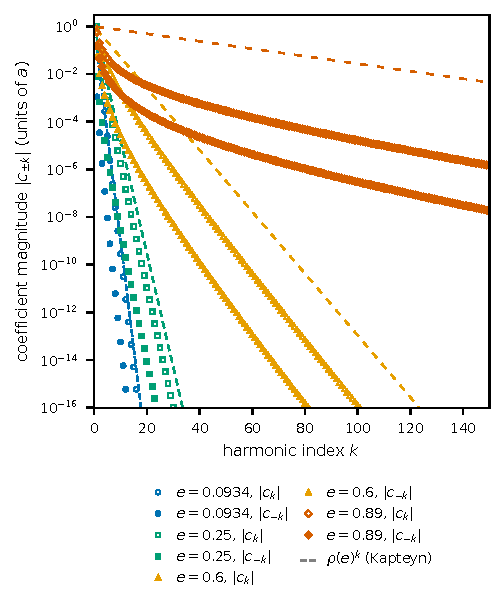
\includegraphics[width=\columnwidth]{fig_coeff_decay.pdf}
\caption{Magnitude of the Kepler-orbit Fourier coefficients $|c_k|$ (open
markers, $k>0$, prograde) and $|c_{-k}|$ (filled markers, retrograde; marker
shape distinguishes $e$) in units of $a$, for $e\in\{0.0934,0.25,0.6,0.89\}$
(Mars, and three illustrative values; $e=0.89$ is Phaethon). Dashed lines:
the Kapteyn rate $\rho(e)^k$.}
\label{fig:decay}
\end{figure}

\subsection{Geocentric convergence}
\label{sec:res-conv}

Figure~\ref{fig:conv} shows the maximum geocentric error over a $50$-yr window
(daily samples) of the truncated chain with $N_{\rm body}=N_\oplus=N$,
against exact Kepler motion, together with the rigorous tail bound
$\varepsilon_N(\text{body})+\varepsilon_N(\oplus)$. The bound is respected
everywhere and the error saturates at the double-precision floor,
$\sim2\times10^{-13}$~AU. The smallest sampled $N$ for which the error is below
$10^{-6}$~AU is $6$ for Mars, $6$ for Ceres and $240$ for Phaethon, and below
$10^{-9}$~AU it is $10$, $10$ and $450$. The cost is therefore
$2N=12$ to $20$ rotating circles plus a static offset per orbit ($24$ to $40$ rotating circles plus one combined offset in the geocentric chain) for planet-like eccentricities and of order a thousand for
$e=0.89$, consistent with the steep growth of the certified order
$N_{\rm cert}\propto(1-e)^{-3/2}$ (not the asymptotic behaviour of the actual
minimal order; Table~\ref{tab:nearpar}). For the single-body series
the observed $N$ for a sup error below $10^{-12}a$ is $12$ for Mars and
$575$ for $e=0.89$, and the analytic bound overestimates it by at most a
factor of $\approx1.5$.

\begin{figure}[H]
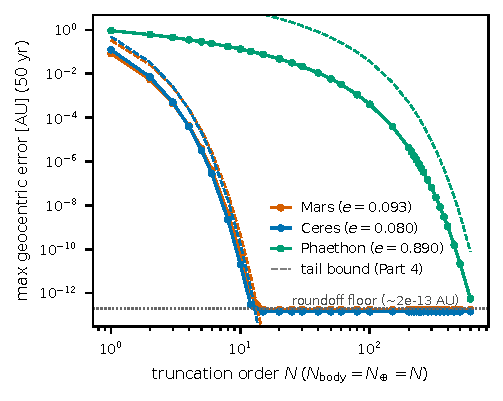
\includegraphics[width=\columnwidth]{fig_geo_convergence.pdf}
\caption{Maximum geocentric position error [AU] over a 50-yr window (daily
samples from JD 2461200.5) of the truncated epicycle chain with
$N_{\rm body}=N_\oplus=N$ versus exact Kepler motion, for Mars, Ceres and
Phaethon (solid), with the rigorous tail bound (dashed). Errors saturate at
the roundoff floor ($\sim2\times10^{-13}$~AU).}
\label{fig:conv}
\end{figure}

\subsection{Low-order truncations of Mars}
\label{sec:res-ptolemy}

Table~\ref{tab:ptolemy} gives the longitude error of truncations of the
geocentric Mars series in the planar approximation (coplanar J2000 mean
elements, $60$ yr at $0.5$~d steps, exact two-body reference, no light time or
aberration). The circular two-term approximation A, a single deferent and a single epicycle
($k=+1$ for both Mars and the Earth) with no eccentric offset and no equant,
reproduces all $28$ retrograde
loops of the true motion, which is the qualitative achievement of the epicycle
construction, but its longitude error reaches $33.2^\circ$ (RMS $9.7^\circ$), at perihelic
oppositions where the true distance is $0.37$~AU against $0.52$~AU in the
circular model. Adding the $k=0$ (eccentric) terms, model B, brings this to
$9.4^\circ$, and the equant-level model C to $5.05^\circ$. None of
these is a literal reproduction of Ptolemy's models, whose eccentric and equant
agree with the $k=0,1,2$ terms only to first order in $e$
\cite{Evans1984,Evans1988}; in particular model A is not Ptolemy's model, and
its $33.2^\circ$ error is not an assessment of Ptolemy's accuracy. The table says what a harmonic truncation of the
same order achieves. Truncation by retained set is not monotone at small
orders (E is slightly worse than D, because the retrograde terms shift errors
that partly cancelled), and a monotone decrease sets in only for
$|k|\le5$, where the error is $6\times10^{-4}$ degrees. The $N=5$ chain
($10+10$ rotating circles plus offsets) is within $0.001^\circ$ over the window of
Fig.~\ref{fig:retro}.

\begin{table}[H]
\caption{Low-order truncations of geocentric Mars (A is the circular two-term
approximation, with no eccentric and no equant), planar approximation,
$60$ years. Longitude error against the exact two-body motion; the true
number of retrograde intervals is $28$ and every model reproduces it.}
\label{tab:ptolemy}
\begin{ruledtabular}
\begin{tabular}{llrr}
Model & Retained terms & max ($^\circ$) & RMS ($^\circ$)\\
\hline
A & $k=1$, both bodies & $33.2$ & $9.7$\\
B & $k\in\{0,1\}$, both & $9.40$ & $2.7$\\
C & Mars $k\in\{0,1,2\}$, Earth $k=1$ & $5.05$ & $0.97$\\
D & $k\in\{0,1,2\}$, both & $0.557$ & $0.159$\\
E & $|k|\le2$, both & $0.728$ & $0.182$\\
F & $|k|\le5$, both & $6\times10^{-4}$ & $1\times10^{-4}$\\
G & $|k|\le10$, both & $<10^{-4}$ & $<10^{-4}$\\
\end{tabular}
\end{ruledtabular}
\end{table}

\begin{figure}[H]
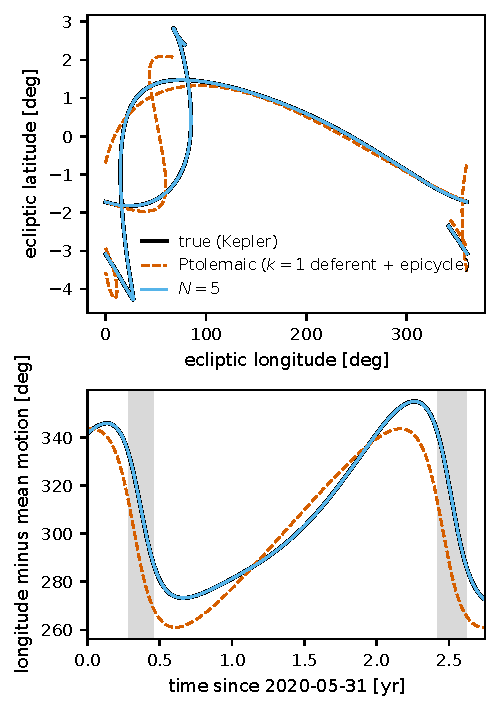
\includegraphics[width=\columnwidth]{fig_mars_retrograde.pdf}
\caption{Geocentric Mars over 2.75 years from 2020-05-31 (two oppositions).
Top: sky track in ecliptic longitude and latitude. Bottom: unwrapped longitude
minus its mean motion ($0.524^\circ$/day); grey bands mark retrograde motion
of the true path. Black: exact Kepler; dashed: circular two-term approximation
(Mars $k=+1$ deferent plus Earth $k=+1$ epicycle only, with no eccentric or
equant, so not Ptolemy's actual model; model A of
Table~\ref{tab:ptolemy}); blue: $N=5$ ($10+10$ rotating circles plus an offset each). The circular two-term approximation
reproduces the retrograde loops but is displaced by up to $32.8^\circ$ in
longitude in this window (planar 60-yr sup norm $33.2^\circ$, RMS
$9.7^\circ$); $N=5$ is within $0.001^\circ$.}
\label{fig:retro}
\end{figure}

\begin{figure}[H]
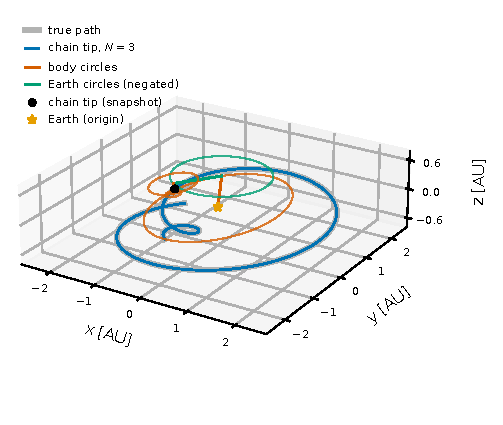
\includegraphics[width=\columnwidth]{fig_chain_3d.pdf}
\caption{Geocentric epicycle chain of Eros (inclination $10.8^\circ$) with
$N=3$ for Eros and for the Earth (12 rotating circles plus the static offsets, each circle drawn in its own orbital
plane about the preceding arm tip; red: body circles, green: negated Earth
circles). Blue: tip trail over one synodic period ($845$~d); grey: exact path.
Maximum tip error $0.01$~AU at this low order.}
\label{fig:chain3d}
\end{figure}

Figure~\ref{fig:chain3d} shows that inclination is handled without
modification: each circle lies in its own orbital plane, and the chain for
Eros ($i=10.8^\circ$) closes onto the exact path with the stated error.

\subsection{NAFF on Keplerian trajectories}
\label{sec:res-naff-kepler}

To validate the extraction we apply NAFF (Sec.~\ref{sec:num-naff}, Hann$^4$
window) to the \emph{exact} Keplerian geocentric Mars series over $200$ yr
sampled every $10$~d with $K=24$ lines, and match the lines to the analytic
Bessel terms. For the ten largest analytic terms the worst relative frequency
error is $2.0\times10^{-10}$ and the worst relative radius error is
$8.9\times10^{-8}$. On a $100$-yr Eros series ($5$-day sampling, $K=40$, $p=4$) the
reconstruction error is $7.6\times10^{-7}$~AU at worst over the full window
(record ends) and $3.1\times10^{-8}$~AU over the interior $80\%$. The data-driven extraction therefore rediscovers the analytic
epicycles; Table~\ref{tab:naff-lines} lists the ten circles with their
individual frequency, radius and phase errors.

\begin{table}[tb]
\caption{The ten largest analytic circles of the Keplerian geocentric Mars chain
($N_{\rm body}=N_\oplus=40$, excluding the static offset) and their recovery by NAFF
($200$ yr, $10$-day sampling, Hann$^4$ window, $K=24$). Circles, not lines:
the prograde and retrograde circles of one harmonic ($\pm k\,n_{\rm M}$) are
recovered from a single NAFF line and so share the same frequency error. $n_{\rm M}$ and
$n_\oplus$ are the mean motions of Mars and the Earth; the retrograde circles
$-k\,n_{\rm M}$ are those with negative index. Errors are relative for frequency and radius and
absolute (rad) for phase. Source: \texttt{experiments/out/naff\_lines\_mars.json}.}
\label{tab:naff-lines}
\begin{ruledtabular}
\footnotesize\setlength{\tabcolsep}{3pt}
\begin{tabular}{lrrrr}
Circle & Radius (AU) & $\delta\omega/\omega$ & $\delta r/r$ & $|\delta\phi|$\\
\hline
$+1 n_{\rm M}$ & 1.52 & $2.0\times10^{-10}$ & $8.9\times10^{-8}$ & $6.6\times10^{-8}$ \\
$+1 n_\oplus$ & 1.00 & $6.0\times10^{-11}$ & $6.5\times10^{-8}$ & $3.8\times10^{-8}$ \\
$+2 n_{\rm M}$ & $7.1\times10^{-2}$ & $2.1\times10^{-11}$ & $3.4\times10^{-8}$ & $1.4\times10^{-8}$ \\
$+2 n_\oplus$ & $8.4\times10^{-3}$ & $1.3\times10^{-11}$ & $1.6\times10^{-14}$ & $1.6\times10^{-8}$ \\
$+3 n_{\rm M}$ & $4.9\times10^{-3}$ & $7.2\times10^{-11}$ & $1.8\times10^{-13}$ & $7.2\times10^{-8}$ \\
$-1 n_{\rm M}$ & $1.7\times10^{-3}$ & $2.0\times10^{-10}$ & $8.9\times10^{-8}$ & $6.6\times10^{-8}$ \\
$+4 n_{\rm M}$ & $4.1\times10^{-4}$ & $1.2\times10^{-14}$ & $5.7\times10^{-13}$ & $7.5\times10^{-12}$ \\
$+3 n_\oplus$ & $1.0\times10^{-4}$ & $9.9\times10^{-11}$ & $2.6\times10^{-12}$ & $1.9\times10^{-7}$ \\
$-2 n_{\rm M}$ & $5.2\times10^{-5}$ & $2.1\times10^{-11}$ & $3.4\times10^{-8}$ & $1.4\times10^{-8}$ \\
$+5 n_{\rm M}$ & $3.7\times10^{-5}$ & $3.3\times10^{-11}$ & $2.0\times10^{-11}$ & $5.4\times10^{-8}$ \\
\end{tabular}
\end{ruledtabular}
\end{table}


\subsection{Perturbed Ceres}
\label{sec:res-ceres}

The Ceres test integrates the Sun, Earth, Jupiter, Saturn and a massless Ceres
over $200$ yr (5-day sampling, Sec.~\ref{sec:num-nbody}). A NAFF chain fitted
directly to the geocentric series would also have to absorb the
perturbations of the Earth, which a Kepler fit of Ceres alone cannot do, and the
NAFF window (Hann$^4$) weights the centre of the record much more strongly than
an unweighted least-squares fit does. To make the comparison like for like we
therefore fit the \emph{heliocentric} integrated Ceres trajectory in every case,
and subtract the \emph{same} integrated Earth trajectory from each reconstruction
before measuring the geocentric error, so that Earth-model error is excluded
from all rows. The Kepler baseline is a six-element least-squares fit, reported
both unweighted and weighted by the same Hann$^4$ window as NAFF (residual
weights $\sqrt w$). Errors are reported over the full window and over the interior
$80\%$ (Sec.~\ref{sec:num-baselines}).

Table~\ref{tab:ceres} gives the result. The interior error of the NAFF chain
decreases overall with the number of lines $K$, from $2.6\times10^{-2}$~AU at
$K=5$ to $1.7\times10^{-5}$~AU at $K=200$ (RMS $2.0\times10^{-6}$~AU). The
decrease is not monotone at the start: the interior maximum rises slightly from
$2.6\times10^{-2}$~AU at $K=5$ to $2.9\times10^{-2}$~AU at $K=10$ and decreases
monotonically for $K\ge10$, while the interior RMS decreases at every step. The NAFF interior maximum is
comparable to the fitted Kepler orbit ($2.7\times10^{-2}$~AU unweighted, RMS
$1.2\times10^{-2}$~AU) at $K=5$--$10$ and clearly smaller only for
$K\gtrsim50$ ($1.1\times10^{-2}$~AU at $K=50$, $1.1\times10^{-3}$~AU at
$K=100$). The full-window error does not fall: it lies between
$2.2\times10^{-2}$ and $4.4\times10^{-2}$~AU for all $K$ and grows with $K$ beyond
$K=20$, because the window vanishes at the record ends and the extra lines fit
the interior at the expense of the edges. The $K=200$ chain is therefore worse in
the maximum norm over the full window ($4.4\times10^{-2}$~AU) than either
Kepler fit ($3.7\times10^{-2}$~AU unweighted, $2.9\times10^{-2}$~AU weighted).
Weighting the Kepler fit by the Hann$^4$ window does not help it in the
interior: its interior maximum is slightly \emph{worse}
($2.8\times10^{-2}$ against $2.7\times10^{-2}$~AU) and only the full-window
maximum improves. Fitting NAFF to the geocentric series directly (the earlier
protocol, Fig.~\ref{fig:ceres}) gives interior errors larger by a factor of about $3$ at $K=200$ ($5.4\times10^{-5}$ against $1.7\times10^{-5}$~AU), and moving the Kepler baseline from the geocentric to the
heliocentric protocol changes its interior maximum only from
$2.74\times10^{-2}$ to $2.67\times10^{-2}$~AU. The comparison therefore does not
hinge on the Earth model, and we do not attribute the NAFF improvement to the
representation of Ceres alone: part of the difference between the two NAFF
protocols is the additional Earth lines that a geocentric fit must carry.
Osculating elements at the epoch give a much larger error, $0.89$~AU, an
artifact of osculating versus mean elements that we do not regard as a
meaningful comparison.

Figure~\ref{fig:ceresres} shows why the full-window and interior numbers
differ. The NAFF residuals are smallest at the centre of the record, rise
gradually towards both ends, and climb steeply within the first and last
$10\%$ to the size of the Kepler residuals, where the Hann$^4$ weight is
negligible and the fit is essentially unconstrained. This is the endpoint
effect, and it worsens as lines are added because they are placed to reduce the
weighted, mostly interior, residual. The Kepler residuals, weighted or not,
oscillate at the $10^{-2}$~AU level across the whole window, being limited by
the perturbation terms that a single ellipse cannot represent; the weighting
reshapes them only slightly.

\begin{table}[tb]
\caption{Perturbed Ceres, $200$ yr: maximum geocentric error [AU] of
reconstructions fitted to the \emph{heliocentric} integrated Ceres trajectory,
with the same integrated Earth subtracted from every row. NAFF with $K$ lines
($2K$ rotating circles plus a static offset), and six-element Kepler fits
unweighted and weighted by the Hann$^4$ window of NAFF.
$^a$Rotating circles, excluding the static offset.}
\label{tab:ceres}
\begin{ruledtabular}
\begin{tabular}{lrrr}
 & circles$^a$ & interior & full\\
\hline
NAFF $K=5$ & 10 & $2.6\times10^{-2}$ & $2.6\times10^{-2}$\\
NAFF $K=20$ & 40 & $1.9\times10^{-2}$ & $2.2\times10^{-2}$\\
NAFF $K=50$ & 100 & $1.1\times10^{-2}$ & $3.0\times10^{-2}$\\
NAFF $K=100$ & 200 & $1.1\times10^{-3}$ & $3.5\times10^{-2}$\\
NAFF $K=200$ & 400 & $1.7\times10^{-5}$ & $4.4\times10^{-2}$\\
Kepler fit, unweighted & 1 orbit & $2.7\times10^{-2}$ & $3.7\times10^{-2}$\\
Kepler fit, Hann$^4$-wtd & 1 orbit & $2.8\times10^{-2}$ & $2.9\times10^{-2}$\\
\end{tabular}
\end{ruledtabular}
\end{table}

\begin{figure}[H]
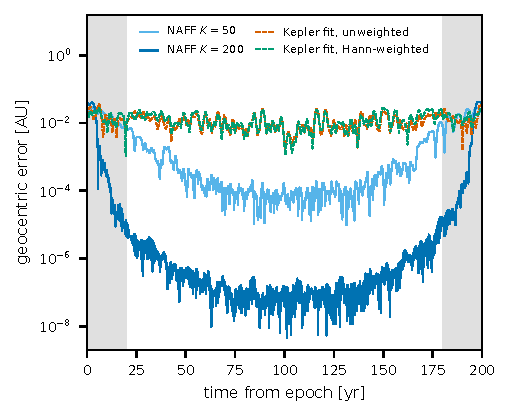
\includegraphics[width=\columnwidth]{fig_ceres_residual_time.pdf}
\caption{Geocentric position error [AU] of reconstructed Ceres versus time over the
$200$-yr N-body window, with the same integrated Earth subtracted from every
reconstruction. NAFF chains ($K=50$, $K=200$) are fitted to heliocentric Ceres
with the Hann$^4$ window; the six-element Kepler fits to heliocentric Ceres are
shown unweighted and weighted by the same window. Grey bands mark the first
and last $10\%$ of the record, outside the interior $80\%$ used for the interior
statistics. The NAFF errors rise towards the window ends, where the window
weight vanishes.}
\label{fig:ceresres}
\end{figure}

\begin{figure}[H]
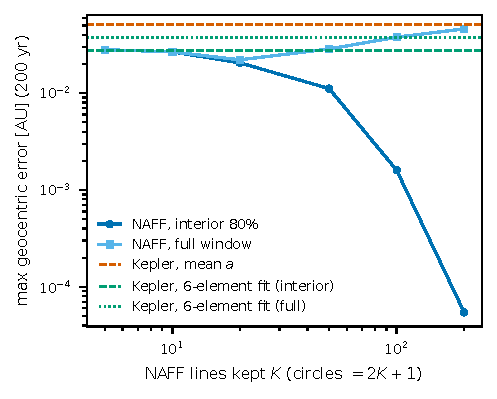
\includegraphics[width=\columnwidth]{fig_perturbed_ceres.pdf}
\caption{Maximum geocentric position error [AU] of a NAFF-extracted epicycle
chain ($2K$ rotating circles plus a static offset) fitted directly to the N-body (Sun, Earth, Jupiter, Saturn)
geocentric Ceres trajectory over 200 years (so Earth's perturbations are
fitted too), versus the number of lines $K$:
interior 80\% of the window (dark blue) and full window (light blue).
Horizontal lines: Kepler baselines that fit only Ceres with the Earth held on a Kepler orbit,
mean-$a$ Kepler $0.051$~AU and
6-element least-squares Kepler fit $0.027$~AU (interior), $0.038$~AU (full).
The osculating-element Kepler orbit (error $0.89$~AU) is omitted as an
element-offset artifact. The matched comparison is Table~\ref{tab:ceres}.}
\label{fig:ceres}
\end{figure}

\section{Visualization}
\label{sec:viz}

\begin{figure*}[t]
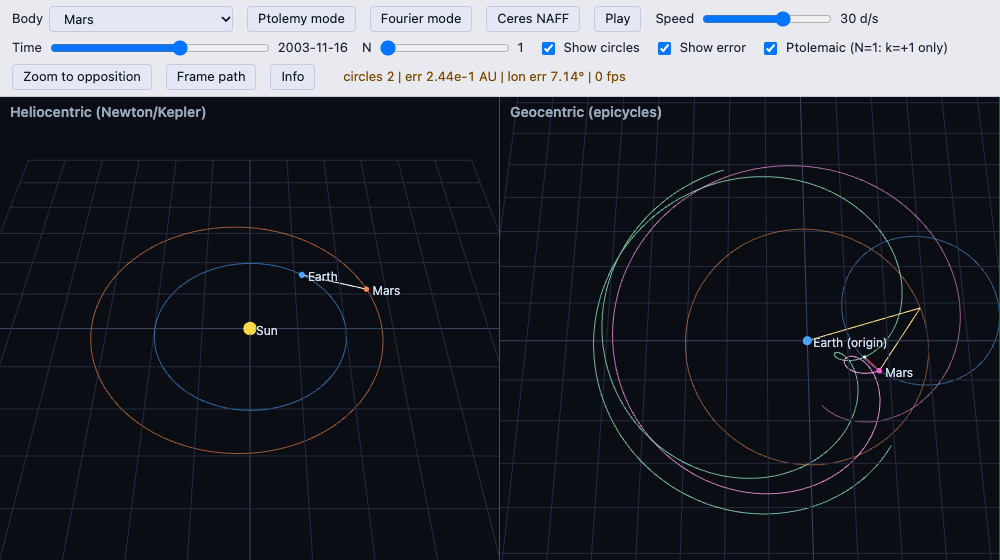
\includegraphics[width=\textwidth]{fig_spa_screenshot.png}
\caption{Screenshot of the interactive viewer (URL parameters
\texttt{preset=ptolemy\&t=2452960\&N=1\&info=0}: Mars, Julian date 2452960,
Ptolemaic $k=+1$ subset only, error shown). Left: heliocentric Newtonian view.
Right: geocentric view with the epicycle chain (yellow arm), its two circles,
the trail of the chain tip, the exact geocentric path (green) and the error
vector (red) between the chain tip and true Mars. The readout (top) shows the
circle count and the error against exact Kepler motion (here $0.244$~AU,
$7.14^\circ$ in longitude).}
\label{fig:spa}
\end{figure*}

To make the construction tangible we provide an open-source interactive
viewer, a single-page web application (TypeScript and three.js) in the
\texttt{web/} directory of the repository. Figure~\ref{fig:spa} shows it. Two
three-dimensional views are synchronized to one clock. The left view is
heliocentric and Newtonian: the Sun, the Earth and the chosen body move on
their Kepler ellipses. The right view is geocentric, centred on the Earth,
and shows the epicycle chain: the deferent, the successive epicycles drawn
as circles in their own orbital planes, the arm joining their centres, and
the trail of the chain tip. In the left panel a line joins the Earth to the body; it is
the geocentric vector whose epicycle sum is drawn in the right panel.

The geocentric chain is computed live in the browser, by a TypeScript port
of the Kepler and Bessel-coefficient code of Sec.~\ref{sec:num-expansion}
that is tested against golden values generated by the Python reference.
Nothing is precomputed or fitted: the radii, planes and angular rates are the
analytic quantities of Sec.~\ref{sec:theory}, determined by the orbital
elements. The slider $N$ ($1$ to $60$) sets the truncation order for both the
body and the Earth, so the viewer demonstrates the convergence of
Sec.~\ref{sec:res-conv} directly: at $N=1$ one sees the Ptolemaic
deferent-and-epicycle picture with its visible displacement, and as $N$
increases the chain tip converges onto the heliocentric truth and the small
circles shrink. A live readout shows the number of circles and the
instantaneous error against exact Kepler motion, in AU and as a
longitude error. The state is encoded in URL parameters (\texttt{t}, a Julian
date, \texttt{N}, \texttt{speed} in days per second, and \texttt{paused}) so that a configuration can be shared.
Intended uses are as a classroom demonstration of what ``epicycles are
Fourier series'' means quantitatively, and of how fast the series converges
for planet-like eccentricities.


\section{Discussion}
\label{sec:discussion}
% TODO: validity domain (bounded quasi-periodic, chaotic finite-time, unbound fails), answer to the epicycles-fit-anything objection
\todo{validity domain (bounded quasi-periodic, chaotic finite-time, unbound fails), answer to the epicycles-fit-anything objection.}

\section{Conclusion}
\label{sec:conclusion}

For a bound Newtonian two-body orbit, the geocentric position of a body
is exactly a sum of two Bessel--Fourier epicycle families whose radii,
planes and rates are determined by the orbital elements. We gave the explicit
three-dimensional expansion with truncation bounds and verified them: $N\approx6$ to $10$ harmonics, i.e.\ $2N=12$ to $20$ rotating circles
plus an offset per orbit, reach $10^{-6}$ to $10^{-9}$~AU for
Mars and Ceres, hundreds are needed at $e=0.89$, and a circular two-term approximation
of Mars (not Ptolemy's actual model) reproduces the retrograde loops but is off by up to
$33^\circ$. Frequency analysis recovers the analytic epicycles from
Keplerian data to $\sim10^{-10}$ in frequency and, for a perturbed Ceres
trajectory, represents the interior of a $200$-yr window with errors below
$10^{-4}$~AU at $K=200$ while remaining edge-limited over the whole window,
where it is no better than a Kepler ellipse fitted to the same heliocentric data with matched weights. The right
statement of the hypothesis is therefore bounded and finite-window:
exact for Kepler motion, almost-periodic for the geocentric view,
exact on analytic invariant tori, an empirical finite-window approximation for
other perturbed motion, and absent for unbound orbits. The accompanying interactive viewer makes the
convergence visible. Natural next steps are validation against a modern
ephemeris, a treatment of edge effects by better windows or extrapolation, and
extension to more bodies.


\begin{acknowledgments}
The author thanks the maintainers of the open-source scientific Python and three.js ecosystems used in this work.
\end{acknowledgments}

\appendix
\section{Bessel and Kapteyn identities}
\label{app:bessel}

We collect the classical identities used in Sec.~\ref{sec:theory}
\cite{Watson1944,Dutka1995}.

\paragraph*{Generating function and Bessel's integral.}
For integer $n$,
\begin{gather}
e^{\ii x\sin\tau}=\sum_{n\in\mathbb Z}J_n(x)e^{\ii n\tau},\notag\\
J_n(x)=\frac1{2\pi}\int_0^{2\pi}e^{\ii(n\tau-x\sin\tau)}\,d\tau,
\label{eq:genfun}
\end{gather}
with $J_{-n}(x)=(-1)^nJ_n(x)=J_n(-x)$; $J_n$ is real for real $x$, and the
integral is unchanged under $\tau\to-\tau$ combined with $n\to-n$ so that the sign
of the exponent in Lemma~\ref{lem:coef} is immaterial. The cosine and sine forms
are
\begin{align}
J_n'(x)&=\frac1\pi\int_0^\pi\sin\tau\,\sin(n\tau-x\sin\tau)\,d\tau,\notag\\
\tfrac12\big[J_{n-1}(x)+J_{n+1}(x)\big]&=\frac1\pi\int_0^\pi\cos\tau\cos(n\tau-x\sin\tau)\,d\tau .
\label{eq:cossin}
\end{align}

\paragraph*{Recurrences.}
Differentiating Eq.~\eqref{eq:genfun} in $x$ and in $\tau$ gives
\begin{align}
J_{n-1}(x)+J_{n+1}(x)&=\frac{2n}{x}J_n(x),\notag\\
J_{n-1}(x)-J_{n+1}(x)&=2J_n'(x),
\label{eq:recur}
\end{align}
and, adding and subtracting,
$J_n'(x)=\frac nxJ_n(x)-J_{n+1}(x)$. At $x=ke$ with $n=k$ the first relation
reads $J_{k-1}(ke)+J_{k+1}(ke)=\tfrac2eJ_k(ke)$, which converts the first form of
Eq.~\eqref{eq:ck} into the derivative-free second form, and, with
$J_k'(ke)=J_k(ke)/e-J_{k+1}(ke)$, gives Eqs.~\eqref{eq:realform}.

\paragraph*{Proof of Lemma~\ref{lem:coef}.}
Since $e^{-\ii kM}dM=d(e^{-\ii kM})/(-\ii k)$, integration by parts gives
\begin{multline}
\frac1{2\pi}\int_0^{2\pi}e^{\ii mE}e^{-\ii kM}dM\\
=\frac{m}{k}\,\frac1{2\pi}\int_0^{2\pi}e^{-\ii[(k-m)E-ke\sin E]}\,dE
=\frac mk\,J_{k-m}(ke),
\end{multline}
using $M=E-e\sin E$ and Eq.~\eqref{eq:genfun}. The boundary term vanishes
because $e^{\ii mE}e^{-\ii kM}$ is $2\pi$-periodic in $M$.

\paragraph*{Kapteyn's inequality.}
For $\nu\ge0$ and $0<\zeta\le1$,
\begin{equation}
|J_\nu(\nu\zeta)|\le\Bigg(\frac{\zeta\,e^{\sqrt{1-\zeta^2}}}{1+\sqrt{1-\zeta^2}}\Bigg)^{\nu}
\label{eq:kapteyn-app}
\end{equation}
is due to Kapteyn \cite{Kapteyn1893}; see Watson \cite{Watson1944}, \S8.7 for
the proof, which is not reproduced here. (We also verified the inequality
numerically for $1\le k\le399$ and $e\in\{0.0167,0.0934,0.25,0.6,0.89,0.99\}$.)
It is the large-order, uniform-in-argument form of the Debye asymptotics
$J_\nu(\nu\,\mathrm{sech}\,\alpha)\sim e^{\nu(\tanh\alpha-\alpha)}/\sqrt{2\pi\nu\tanh\alpha}$
with $\zeta=\mathrm{sech}\,\alpha$, which shows that the geometric rate
$\rho^k$ in Eq.~\eqref{eq:kapteyn} is sharp up to a factor of order
$k^{-1/2}$ for fixed $e$.

\paragraph*{Small-$e$ limits of $c_k$.}
From the series $J_n(x)=\sum_{m\ge0}\frac{(-1)^m}{m!\,(m+n)!}(x/2)^{2m+n}$ one has
$J_k(ke)=\frac{(ke/2)^k}{k!}\big[1-\frac{(ke/2)^2}{k+1}+\dots\big]$, so
$J_k(ke)=O(e^k)$ and $J_{k+1}(ke)=O(e^{k+1})$. With $(1+s)/e=2/e-e/2+\dots$ and
$(1-s)/e=e/2+\dots$ in Eqs.~\eqref{eq:ck}--\eqref{eq:cmk}:
\begin{gather}
c_k=\frac{k^{k-1}}{2^{k-1}\,k!}\,e^{k-1}\big[1+O(e^2)\big],\notag\\
c_{-k}=O(e^{k+1}),\qquad k\ge1.
\label{eq:cksmall}
\end{gather}
In particular $c_1\to1$, $c_2\sim e/2$, $c_3\sim 3e^2/8$, and
$c_{-1}\sim e^2/8$, $c_{-2}\sim e^3/24$ (Eq.~\eqref{eq:smalle}), and
every coefficient is finite as $e\to0$ although individual factors $1/e$ in
Eq.~\eqref{eq:ck} are not. Retrograde circles are thus smaller than the corresponding
prograde ones by a factor $O(e^2)$ at small $k$ (e.g.\ $|c_{-1}/c_1|\sim e^2/8$).


\bibliography{refs}

\end{document}
